% Created by tikzDevice version 0.12.3.1 on 2021-04-15 15:43:15
% !TEX encoding = UTF-8 Unicode
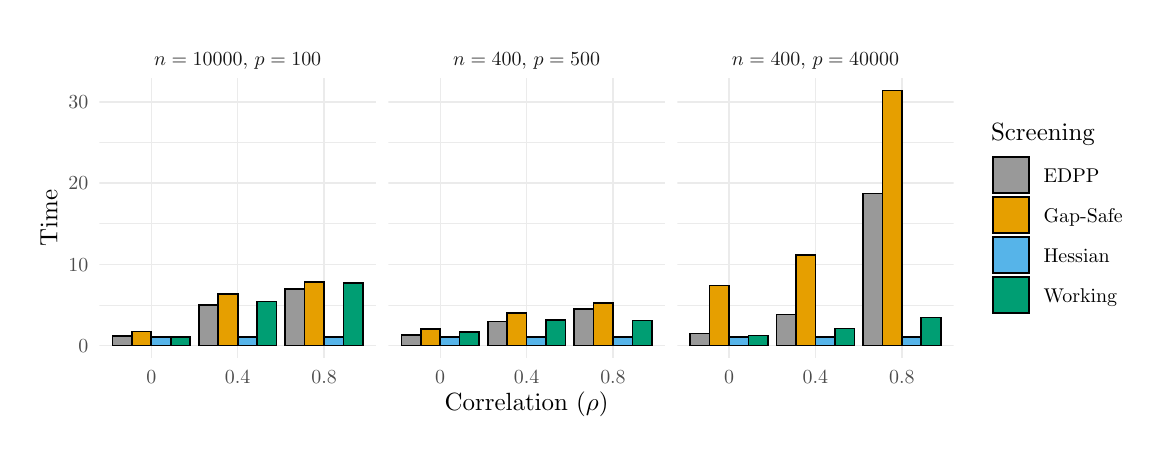
\begin{tikzpicture}[x=1pt,y=1pt]
\definecolor{fillColor}{RGB}{255,255,255}
\path[use as bounding box,fill=fillColor,fill opacity=0.00] (0,0) rectangle (404.71,144.54);
\begin{scope}
\path[clip] ( 25.95, 25.11) rectangle (125.84,126.48);
\definecolor{drawColor}{gray}{0.92}

\path[draw=drawColor,line width= 0.2pt,line join=round] ( 25.95, 44.38) --
	(125.84, 44.38);

\path[draw=drawColor,line width= 0.2pt,line join=round] ( 25.95, 73.71) --
	(125.84, 73.71);

\path[draw=drawColor,line width= 0.2pt,line join=round] ( 25.95,103.04) --
	(125.84,103.04);

\path[draw=drawColor,line width= 0.5pt,line join=round] ( 25.95, 29.71) --
	(125.84, 29.71);

\path[draw=drawColor,line width= 0.5pt,line join=round] ( 25.95, 59.05) --
	(125.84, 59.05);

\path[draw=drawColor,line width= 0.5pt,line join=round] ( 25.95, 88.38) --
	(125.84, 88.38);

\path[draw=drawColor,line width= 0.5pt,line join=round] ( 25.95,117.71) --
	(125.84,117.71);

\path[draw=drawColor,line width= 0.5pt,line join=round] ( 44.68, 25.11) --
	( 44.68,126.48);

\path[draw=drawColor,line width= 0.5pt,line join=round] ( 75.89, 25.11) --
	( 75.89,126.48);

\path[draw=drawColor,line width= 0.5pt,line join=round] (107.11, 25.11) --
	(107.11,126.48);
\definecolor{drawColor}{RGB}{0,0,0}
\definecolor{fillColor}{gray}{0.60}

\path[draw=drawColor,line width= 0.6pt,line cap=rect,fill=fillColor] ( 30.63, 29.71) rectangle ( 37.65, 33.11);
\definecolor{fillColor}{RGB}{230,159,0}

\path[draw=drawColor,line width= 0.6pt,line cap=rect,fill=fillColor] ( 37.65, 29.71) rectangle ( 44.68, 34.75);
\definecolor{fillColor}{RGB}{86,180,233}

\path[draw=drawColor,line width= 0.6pt,line cap=rect,fill=fillColor] ( 44.68, 29.71) rectangle ( 51.70, 32.65);
\definecolor{fillColor}{RGB}{0,158,115}

\path[draw=drawColor,line width= 0.6pt,line cap=rect,fill=fillColor] ( 51.70, 29.71) rectangle ( 58.72, 32.73);
\definecolor{fillColor}{gray}{0.60}

\path[draw=drawColor,line width= 0.6pt,line cap=rect,fill=fillColor] ( 61.84, 29.71) rectangle ( 68.87, 44.37);
\definecolor{fillColor}{RGB}{230,159,0}

\path[draw=drawColor,line width= 0.6pt,line cap=rect,fill=fillColor] ( 68.87, 29.71) rectangle ( 75.89, 48.19);
\definecolor{fillColor}{RGB}{86,180,233}

\path[draw=drawColor,line width= 0.6pt,line cap=rect,fill=fillColor] ( 75.89, 29.71) rectangle ( 82.91, 32.65);
\definecolor{fillColor}{RGB}{0,158,115}

\path[draw=drawColor,line width= 0.6pt,line cap=rect,fill=fillColor] ( 82.91, 29.71) rectangle ( 89.94, 45.63);
\definecolor{fillColor}{gray}{0.60}

\path[draw=drawColor,line width= 0.6pt,line cap=rect,fill=fillColor] ( 93.06, 29.71) rectangle (100.08, 50.05);
\definecolor{fillColor}{RGB}{230,159,0}

\path[draw=drawColor,line width= 0.6pt,line cap=rect,fill=fillColor] (100.08, 29.71) rectangle (107.11, 52.58);
\definecolor{fillColor}{RGB}{86,180,233}

\path[draw=drawColor,line width= 0.6pt,line cap=rect,fill=fillColor] (107.11, 29.71) rectangle (114.13, 32.65);
\definecolor{fillColor}{RGB}{0,158,115}

\path[draw=drawColor,line width= 0.6pt,line cap=rect,fill=fillColor] (114.13, 29.71) rectangle (121.15, 52.24);
\end{scope}
\begin{scope}
\path[clip] (130.34, 25.11) rectangle (230.23,126.48);
\definecolor{drawColor}{gray}{0.92}

\path[draw=drawColor,line width= 0.2pt,line join=round] (130.34, 44.38) --
	(230.23, 44.38);

\path[draw=drawColor,line width= 0.2pt,line join=round] (130.34, 73.71) --
	(230.23, 73.71);

\path[draw=drawColor,line width= 0.2pt,line join=round] (130.34,103.04) --
	(230.23,103.04);

\path[draw=drawColor,line width= 0.5pt,line join=round] (130.34, 29.71) --
	(230.23, 29.71);

\path[draw=drawColor,line width= 0.5pt,line join=round] (130.34, 59.05) --
	(230.23, 59.05);

\path[draw=drawColor,line width= 0.5pt,line join=round] (130.34, 88.38) --
	(230.23, 88.38);

\path[draw=drawColor,line width= 0.5pt,line join=round] (130.34,117.71) --
	(230.23,117.71);

\path[draw=drawColor,line width= 0.5pt,line join=round] (149.07, 25.11) --
	(149.07,126.48);

\path[draw=drawColor,line width= 0.5pt,line join=round] (180.28, 25.11) --
	(180.28,126.48);

\path[draw=drawColor,line width= 0.5pt,line join=round] (211.50, 25.11) --
	(211.50,126.48);
\definecolor{drawColor}{RGB}{0,0,0}
\definecolor{fillColor}{gray}{0.60}

\path[draw=drawColor,line width= 0.6pt,line cap=rect,fill=fillColor] (135.02, 29.71) rectangle (142.04, 33.56);
\definecolor{fillColor}{RGB}{230,159,0}

\path[draw=drawColor,line width= 0.6pt,line cap=rect,fill=fillColor] (142.04, 29.71) rectangle (149.07, 35.64);
\definecolor{fillColor}{RGB}{86,180,233}

\path[draw=drawColor,line width= 0.6pt,line cap=rect,fill=fillColor] (149.07, 29.71) rectangle (156.09, 32.65);
\definecolor{fillColor}{RGB}{0,158,115}

\path[draw=drawColor,line width= 0.6pt,line cap=rect,fill=fillColor] (156.09, 29.71) rectangle (163.11, 34.56);
\definecolor{fillColor}{gray}{0.60}

\path[draw=drawColor,line width= 0.6pt,line cap=rect,fill=fillColor] (166.23, 29.71) rectangle (173.26, 38.36);
\definecolor{fillColor}{RGB}{230,159,0}

\path[draw=drawColor,line width= 0.6pt,line cap=rect,fill=fillColor] (173.26, 29.71) rectangle (180.28, 41.49);
\definecolor{fillColor}{RGB}{86,180,233}

\path[draw=drawColor,line width= 0.6pt,line cap=rect,fill=fillColor] (180.28, 29.71) rectangle (187.30, 32.65);
\definecolor{fillColor}{RGB}{0,158,115}

\path[draw=drawColor,line width= 0.6pt,line cap=rect,fill=fillColor] (187.30, 29.71) rectangle (194.33, 38.89);
\definecolor{fillColor}{gray}{0.60}

\path[draw=drawColor,line width= 0.6pt,line cap=rect,fill=fillColor] (197.45, 29.71) rectangle (204.47, 42.88);
\definecolor{fillColor}{RGB}{230,159,0}

\path[draw=drawColor,line width= 0.6pt,line cap=rect,fill=fillColor] (204.47, 29.71) rectangle (211.50, 45.15);
\definecolor{fillColor}{RGB}{86,180,233}

\path[draw=drawColor,line width= 0.6pt,line cap=rect,fill=fillColor] (211.50, 29.71) rectangle (218.52, 32.65);
\definecolor{fillColor}{RGB}{0,158,115}

\path[draw=drawColor,line width= 0.6pt,line cap=rect,fill=fillColor] (218.52, 29.71) rectangle (225.54, 38.74);
\end{scope}
\begin{scope}
\path[clip] (234.73, 25.11) rectangle (334.61,126.48);
\definecolor{drawColor}{gray}{0.92}

\path[draw=drawColor,line width= 0.2pt,line join=round] (234.73, 44.38) --
	(334.61, 44.38);

\path[draw=drawColor,line width= 0.2pt,line join=round] (234.73, 73.71) --
	(334.61, 73.71);

\path[draw=drawColor,line width= 0.2pt,line join=round] (234.73,103.04) --
	(334.61,103.04);

\path[draw=drawColor,line width= 0.5pt,line join=round] (234.73, 29.71) --
	(334.61, 29.71);

\path[draw=drawColor,line width= 0.5pt,line join=round] (234.73, 59.05) --
	(334.61, 59.05);

\path[draw=drawColor,line width= 0.5pt,line join=round] (234.73, 88.38) --
	(334.61, 88.38);

\path[draw=drawColor,line width= 0.5pt,line join=round] (234.73,117.71) --
	(334.61,117.71);

\path[draw=drawColor,line width= 0.5pt,line join=round] (253.45, 25.11) --
	(253.45,126.48);

\path[draw=drawColor,line width= 0.5pt,line join=round] (284.67, 25.11) --
	(284.67,126.48);

\path[draw=drawColor,line width= 0.5pt,line join=round] (315.89, 25.11) --
	(315.89,126.48);
\definecolor{drawColor}{RGB}{0,0,0}
\definecolor{fillColor}{gray}{0.60}

\path[draw=drawColor,line width= 0.6pt,line cap=rect,fill=fillColor] (239.41, 29.71) rectangle (246.43, 34.02);
\definecolor{fillColor}{RGB}{230,159,0}

\path[draw=drawColor,line width= 0.6pt,line cap=rect,fill=fillColor] (246.43, 29.71) rectangle (253.45, 51.39);
\definecolor{fillColor}{RGB}{86,180,233}

\path[draw=drawColor,line width= 0.6pt,line cap=rect,fill=fillColor] (253.45, 29.71) rectangle (260.48, 32.65);
\definecolor{fillColor}{RGB}{0,158,115}

\path[draw=drawColor,line width= 0.6pt,line cap=rect,fill=fillColor] (260.48, 29.71) rectangle (267.50, 33.34);
\definecolor{fillColor}{gray}{0.60}

\path[draw=drawColor,line width= 0.6pt,line cap=rect,fill=fillColor] (270.62, 29.71) rectangle (277.65, 40.85);
\definecolor{fillColor}{RGB}{230,159,0}

\path[draw=drawColor,line width= 0.6pt,line cap=rect,fill=fillColor] (277.65, 29.71) rectangle (284.67, 62.51);
\definecolor{fillColor}{RGB}{86,180,233}

\path[draw=drawColor,line width= 0.6pt,line cap=rect,fill=fillColor] (284.67, 29.71) rectangle (291.69, 32.65);
\definecolor{fillColor}{RGB}{0,158,115}

\path[draw=drawColor,line width= 0.6pt,line cap=rect,fill=fillColor] (291.69, 29.71) rectangle (298.72, 35.87);
\definecolor{fillColor}{gray}{0.60}

\path[draw=drawColor,line width= 0.6pt,line cap=rect,fill=fillColor] (301.84, 29.71) rectangle (308.86, 84.62);
\definecolor{fillColor}{RGB}{230,159,0}

\path[draw=drawColor,line width= 0.6pt,line cap=rect,fill=fillColor] (308.86, 29.71) rectangle (315.89,121.87);
\definecolor{fillColor}{RGB}{86,180,233}

\path[draw=drawColor,line width= 0.6pt,line cap=rect,fill=fillColor] (315.89, 29.71) rectangle (322.91, 32.65);
\definecolor{fillColor}{RGB}{0,158,115}

\path[draw=drawColor,line width= 0.6pt,line cap=rect,fill=fillColor] (322.91, 29.71) rectangle (329.93, 39.78);
\end{scope}
\begin{scope}
\path[clip] ( 25.95,126.48) rectangle (125.84,140.04);
\definecolor{drawColor}{gray}{0.10}

\node[text=drawColor,anchor=base,inner sep=0pt, outer sep=0pt, scale=  0.72] at ( 75.89,130.78) {$n=10000$, $p=100$};
\end{scope}
\begin{scope}
\path[clip] (130.34,126.48) rectangle (230.23,140.04);
\definecolor{drawColor}{gray}{0.10}

\node[text=drawColor,anchor=base,inner sep=0pt, outer sep=0pt, scale=  0.72] at (180.28,130.78) {$n=400$, $p=500$};
\end{scope}
\begin{scope}
\path[clip] (234.73,126.48) rectangle (334.61,140.04);
\definecolor{drawColor}{gray}{0.10}

\node[text=drawColor,anchor=base,inner sep=0pt, outer sep=0pt, scale=  0.72] at (284.67,130.78) {$n=400$, $p=40000$};
\end{scope}
\begin{scope}
\path[clip] (  0.00,  0.00) rectangle (404.71,144.54);
\definecolor{drawColor}{gray}{0.30}

\node[text=drawColor,anchor=base,inner sep=0pt, outer sep=0pt, scale=  0.72] at ( 44.68, 16.10) {0};

\node[text=drawColor,anchor=base,inner sep=0pt, outer sep=0pt, scale=  0.72] at ( 75.89, 16.10) {0.4};

\node[text=drawColor,anchor=base,inner sep=0pt, outer sep=0pt, scale=  0.72] at (107.11, 16.10) {0.8};
\end{scope}
\begin{scope}
\path[clip] (  0.00,  0.00) rectangle (404.71,144.54);
\definecolor{drawColor}{gray}{0.30}

\node[text=drawColor,anchor=base,inner sep=0pt, outer sep=0pt, scale=  0.72] at (149.07, 16.10) {0};

\node[text=drawColor,anchor=base,inner sep=0pt, outer sep=0pt, scale=  0.72] at (180.28, 16.10) {0.4};

\node[text=drawColor,anchor=base,inner sep=0pt, outer sep=0pt, scale=  0.72] at (211.50, 16.10) {0.8};
\end{scope}
\begin{scope}
\path[clip] (  0.00,  0.00) rectangle (404.71,144.54);
\definecolor{drawColor}{gray}{0.30}

\node[text=drawColor,anchor=base,inner sep=0pt, outer sep=0pt, scale=  0.72] at (253.45, 16.10) {0};

\node[text=drawColor,anchor=base,inner sep=0pt, outer sep=0pt, scale=  0.72] at (284.67, 16.10) {0.4};

\node[text=drawColor,anchor=base,inner sep=0pt, outer sep=0pt, scale=  0.72] at (315.89, 16.10) {0.8};
\end{scope}
\begin{scope}
\path[clip] (  0.00,  0.00) rectangle (404.71,144.54);
\definecolor{drawColor}{gray}{0.30}

\node[text=drawColor,anchor=base east,inner sep=0pt, outer sep=0pt, scale=  0.72] at ( 21.90, 27.24) {0};

\node[text=drawColor,anchor=base east,inner sep=0pt, outer sep=0pt, scale=  0.72] at ( 21.90, 56.57) {10};

\node[text=drawColor,anchor=base east,inner sep=0pt, outer sep=0pt, scale=  0.72] at ( 21.90, 85.90) {20};

\node[text=drawColor,anchor=base east,inner sep=0pt, outer sep=0pt, scale=  0.72] at ( 21.90,115.23) {30};
\end{scope}
\begin{scope}
\path[clip] (  0.00,  0.00) rectangle (404.71,144.54);
\definecolor{drawColor}{RGB}{0,0,0}

\node[text=drawColor,anchor=base,inner sep=0pt, outer sep=0pt, scale=  0.90] at (180.28,  6.25) {Correlation ($\rho$)};
\end{scope}
\begin{scope}
\path[clip] (  0.00,  0.00) rectangle (404.71,144.54);
\definecolor{drawColor}{RGB}{0,0,0}

\node[text=drawColor,rotate= 90.00,anchor=base,inner sep=0pt, outer sep=0pt, scale=  0.90] at ( 10.70, 75.79) {Time};
\end{scope}
\begin{scope}
\path[clip] (  0.00,  0.00) rectangle (404.71,144.54);
\definecolor{drawColor}{RGB}{0,0,0}

\node[text=drawColor,anchor=base west,inner sep=0pt, outer sep=0pt, scale=  0.90] at (348.11,103.85) {Screening};
\end{scope}
\begin{scope}
\path[clip] (  0.00,  0.00) rectangle (404.71,144.54);
\definecolor{drawColor}{RGB}{0,0,0}
\definecolor{fillColor}{gray}{0.60}

\path[draw=drawColor,line width= 0.6pt,line cap=rect,fill=fillColor] (348.83, 84.74) rectangle (361.86, 97.77);
\end{scope}
\begin{scope}
\path[clip] (  0.00,  0.00) rectangle (404.71,144.54);
\definecolor{drawColor}{RGB}{0,0,0}
\definecolor{fillColor}{RGB}{230,159,0}

\path[draw=drawColor,line width= 0.6pt,line cap=rect,fill=fillColor] (348.83, 70.28) rectangle (361.86, 83.31);
\end{scope}
\begin{scope}
\path[clip] (  0.00,  0.00) rectangle (404.71,144.54);
\definecolor{drawColor}{RGB}{0,0,0}
\definecolor{fillColor}{RGB}{86,180,233}

\path[draw=drawColor,line width= 0.6pt,line cap=rect,fill=fillColor] (348.83, 55.83) rectangle (361.86, 68.86);
\end{scope}
\begin{scope}
\path[clip] (  0.00,  0.00) rectangle (404.71,144.54);
\definecolor{drawColor}{RGB}{0,0,0}
\definecolor{fillColor}{RGB}{0,158,115}

\path[draw=drawColor,line width= 0.6pt,line cap=rect,fill=fillColor] (348.83, 41.37) rectangle (361.86, 54.40);
\end{scope}
\begin{scope}
\path[clip] (  0.00,  0.00) rectangle (404.71,144.54);
\definecolor{drawColor}{RGB}{0,0,0}

\node[text=drawColor,anchor=base west,inner sep=0pt, outer sep=0pt, scale=  0.72] at (367.07, 88.77) {EDPP};
\end{scope}
\begin{scope}
\path[clip] (  0.00,  0.00) rectangle (404.71,144.54);
\definecolor{drawColor}{RGB}{0,0,0}

\node[text=drawColor,anchor=base west,inner sep=0pt, outer sep=0pt, scale=  0.72] at (367.07, 74.32) {Gap-Safe};
\end{scope}
\begin{scope}
\path[clip] (  0.00,  0.00) rectangle (404.71,144.54);
\definecolor{drawColor}{RGB}{0,0,0}

\node[text=drawColor,anchor=base west,inner sep=0pt, outer sep=0pt, scale=  0.72] at (367.07, 59.86) {Hessian};
\end{scope}
\begin{scope}
\path[clip] (  0.00,  0.00) rectangle (404.71,144.54);
\definecolor{drawColor}{RGB}{0,0,0}

\node[text=drawColor,anchor=base west,inner sep=0pt, outer sep=0pt, scale=  0.72] at (367.07, 45.41) {Working};
\end{scope}
\end{tikzpicture}
